\documentclass{article}
\usepackage[utf8]{inputenc}
\usepackage[margin=1in]{geometry}
\usepackage{amsmath,amsthm,amssymb}
\usepackage{natbib}
\usepackage{graphicx}
\usepackage{enumerate}
\usepackage{hyperref}
\usepackage{float}
\usepackage{subcaption}
\usepackage[english]{babel}
\usepackage[T1]{fontenc}
\usepackage{booktabs}
\usepackage{pgf,tikz,pgfplots}
\pgfplotsset{compat=1.15}
\usepackage{mathtools}
\usetikzlibrary{arrows}
\pagestyle{empty}
\usepackage{geometry}
\geometry{margin=1.0in}
\usepackage{verbatim}
\pagestyle{plain}
\usepackage{indentfirst}
\usepackage{wrapfig}
\usepackage{lipsum} 
\setlength\parindent{0pt}
\usepackage{abstract}
\usepackage{sidecap}

\begin{document}

\begin{titlepage}
    \centering
    
\includegraphics[width=10cm]{mcgill}
    \vfill
    \vfill
    {\bfseries\Large
        NeurIPS REPRODUCIBILITY CHALLENGE\\
        ABLATION TRACK\\

        \vskip2cm
        By\\
        Gabriel ALACCHI,\\ 
        Guillaume LAM,\\ 
        Carl PERREAULT-LAFLEUR\\
    }
    \vfill
    Fall 2019
    \vfill
    \vfill
    \vfill
    \vfill
    \vfill
    
\includegraphics[width=10cm]{school_cs_mcgill}
\end{titlepage}
\newpage
\begin{abstract}
In this study, we performed some ablations on the main model developed in the paper "Unsupervised Representation Learning in
Atari" \cite{main_article} as part of the 2019 NeurIPS Reproducibility Challenge. In this paper, Anand et. al introduce a new learning method called SpatioTemporal DeepInfoMax (STDIM), which is an unsupervised method that aims at learning state representations by maximizing particular forms of mutual information between a series of observations. Our work focuses on recreating a subset of their results, along with hyperparameter tuning, slightly altering the STDIM learning objective, and altering the receptive field of the encoder model that Anand et. al introduce in their article. We also suggest directions for further expanding the STDIM method. Our results also suggest that creating an ensemble model would allow for further boosting of the effectiveness of this model.

\end{abstract}

\section{Introduction}
In recent years, reinforcement learning has become an active field of research in the learning algorithms field. It consists of building models which learn how to act and perform tasks in an environment based on past experience. The training of the artificial agents is the main challenge in the production of such algorithms. State representation learning consists of learning to capture the variation in the environment generated by the agent's actions. Hence, state representation learning is crucial for building efficient and powerful agents. The studied article focuses on learning such representations without supervision from rewards. In the article, Anand et. al introduce a new method that learns state representations, called SpatioTemporal DeepInfoMax (STDIM). Furthermore, they also introduce a new benchmark based on 22 Atari 2600 games where it becomes possible to evaluate representations based on how well they capture the ground truth state variables of the game. This allows them to compare STDIM to other state-of-the-art representation learning methods.
\\\\
Section \ref{section:summary} summarizes the studied article to demonstrate the various components our work builds upon. Afterwards, a small subset of the results obtained in the article was reproduced. The ablations performed on STDIM are then summarized. We first experimented with tweaking of the various hyper parameters of the model. This study demonstrates that overall, the default parameters used by the authors of the article are well chosen. The second ablation realized was changing the details of the loss function of STDIM. Our final ablation was changing the encoder to modify the receptive field size that it observes on the input image. The obtained results validate the choices made by the authors and show the robustness of their STDIM method.

\section{Summary of the Article}
\label{section:summary}

\subsection{Objective and Setup}
The setup is fairly simple, an agent interacts with the environment and realizes some observations. The objective of the article for the agent is to learn the representations of the observations such that high-level features in the environment are captured in an unsupervised setting. As shown in Figure \ref{fig:objective}, the aim is to identify the locations of variables such as the player character, enemies, and various of items of interest. It is desired that the model ignores immutable low-level details like the background, which are useless to an agent's ability to process the environment.

\begin{figure}[H]
    \centering
    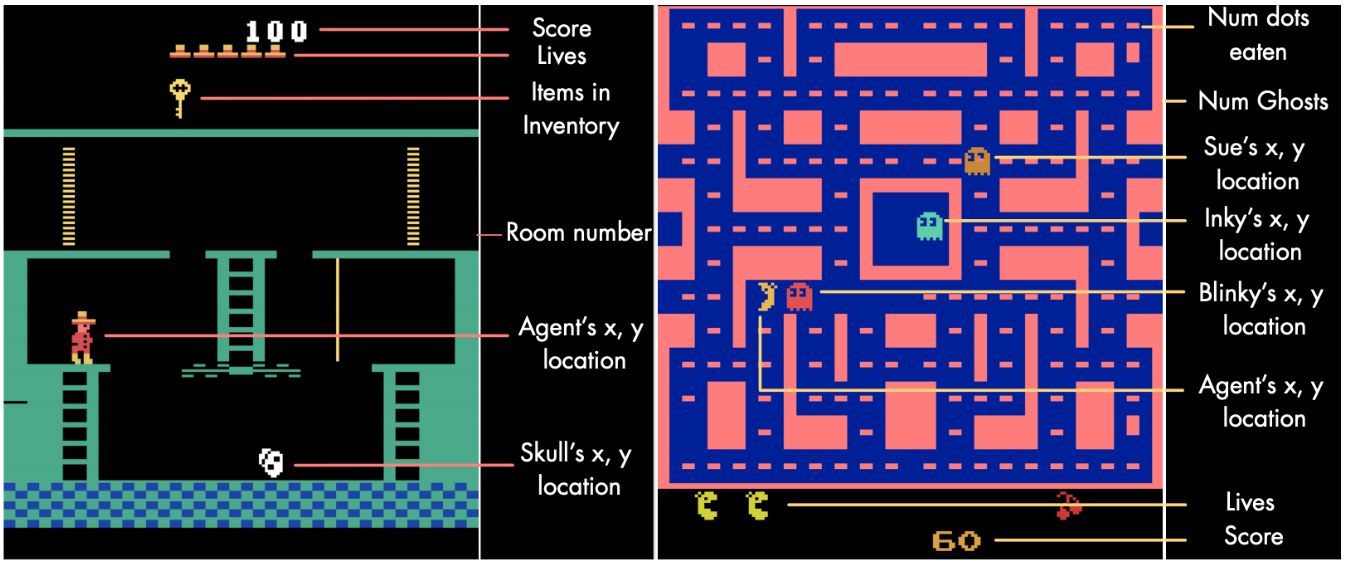
\includegraphics[scale=0.32]{objective.PNG}
    \caption{Objective of a representation learning method}
    \label{fig:objective}
\end{figure}

In order to evaluate a representation learning method after it has been trained, the weights are frozen and then the performance is evaluated with a linear probing task in a supervised manner \cite{linear_probing}. It should be noted that the gradients of the supervised task are not propagated through the encoder. In order to perform well, the encoder must be able to learn \textbf{linearly predictable} representations of crucial variables in the game without supervision.

\subsection{The SpatioTemporal DeepInfoMax (STDIM)}
\label{section:stdim}

\subsubsection{The InfoNCE Objective}

The methods introduced by Anand et. al \cite{main_article} rely on the InfoNCE mutual information bound \cite{infoNCE}. Generally speaking we are given a set of samples $\{(x_i, y_i)\}_{i=1}^{M}$ drawn from a distribution $p(x, y)$. Samples $(x_i, y_i)$ are considered positive samples since they are drawn from the joint probability distribution. Samples which are not indexed the same, i.e. $(x_i, y_j)$ for $i\neq j$ are considered negative samples since they are drawn independently from the marginal distributions, i.e. $Pr(x_i, y_j)=p(x_i)p(y_j)$. The InfoNCE objective is to learn a score function $f$ which maximizes the following estimate which acts as a lower bound of the mutual information between $X$ and $Y$.

\begin{equation}
\mathcal{I}_{NCE}=\sum_{i=1}^N\log{\frac{\exp{f(x_i,y_i)}}{\sum\limits_{\substack{j=1}}^N \exp{f(x_i,y_j)}}}
\label{eqn:info-nce}
\end{equation}

To maximize this bound, $f$ must assign positive values to positive samples, and negative values to negative samples.

\subsubsection{The STDIM Learning Objective}
SpatioTemporal DeepInfoMax (STDIM) is an unsupervised technique for training an encoder network in an unsupervised manner. It builds on the idea of DeepInfoMax (DIM, \cite{DIM}) by maximizing the mutual information (MI) between the representation of consecutive frames by the neural network encoder.
\\\\
An agent interacts with an environment and observes a set of frames $\{x_1, x_2,...,x_n\}$ which generally can be any information which represents the state of the game, but in practice are images from the simulated Atari environment. The InfoNCE objective is derived from mini-batches of consecutive observations $\{(x_t,x_{t+1})_i\}_{i=1}^{B}$ given by the agent's interactions with the environment. Positive samples are defined as pairs of consecutive frames $(x_t,x_{t+1})$, and negative samples as pairs of non-consecutive frames $(x_t,x_{t^\star})$ with $t^\star\ne t+1$. \\

STDIM simultaneously trains two InfoNCE objectives, the global-local objective (GL) and the local-local objective (LL). GL maximizes the MI between the entire frame $x_t$ with small patches of the frame observation at time $t+1$. The representations of the small image patches are chosen to be the result of applying the hidden activation functions of a particular layer of the convolutional encoder to the full observation. The layer is picked appropriately to ensure that the hidden activation functions only have a limited receptive field corresponding to $1/16^{\text{th}}$ the size of the full observations. LL maximizes the MI between the local feature at time $t$ with the corresponding local feature at time $t+1$. The loss function derived from equation \ref{eqn:info-nce} is given by:
\begin{equation}
\mathcal{L}=\mathcal{L}_{GL}+\mathcal{L}_{LL}=\sum_{m=1}^M\sum_{n=1}^N-\left(\log{\frac{\exp{g_{m,n}(x_t,x_{t+1})}}{\sum\limits_{\substack{x_t^\star}} \exp{g_{m,n}(x_t,x_t^\star)}}}+\log{\frac{\exp{f_{m,n}(x_t,x_{t+1})}}{\sum\limits_{\substack{x_t^\star}} \exp{f_{m,n}(x_t,x_t^\star)}}}\right)
\label{eqn:loss-functions}
\end{equation}
where $x_t^\star$ denotes a non-consecutive observation to $x_t$, and $g_{m,n}$ and $f_{m,n}$ are the score functions for the Global-Local and Local-Local objectives respectively. Following the work of van den Oord \cite{infoNCE} on InfoNCE, STDIM uses a bilinear score function for both of these objectives: 
\begin{equation}
g_{m,n}(x_t, x_{t'}) = \phi(x_t)^T \cdot W_g \cdot \phi_{m,n}(x_{t'})\text{ and }  f_{m,n}(x_t, x_{t'}) = \phi_{m,n}(x_t)^T\cdot W_l\cdot \phi_{m,n}(x_{t'})
\label{eqn:bilinear}
\end{equation}
where $\phi$ is the output of the encoder, $\phi_{m,n}$ is the local feature vector produced by an intermediate convolution layer of the encoder at the $(m,n)$ spatial location, and $W_g,W_l$ are learned weights. When training an encoder using these objectives, $W_g$ and $W_l$ are learned to find the maximum for each InfoNCE bound. At run-time these score function weights are discarded since the final objective of this technique is to learn the encoder $\phi$ which creates linearly interpretable representations of the important variables in the game.
\\\\
The base encoder architecture used for all models in the article is shown in Figure \ref{fig:base-encoder-image}.
\begin{figure}[H]
    \centering
    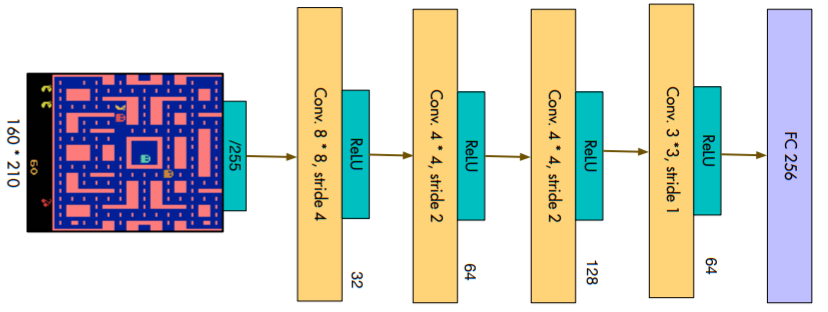
\includegraphics[scale=0.75]{base_encoder.PNG}
    \caption{The base encoder from the article.}
    \label{fig:base-encoder-image}
\end{figure}

\subsection{Linear Probing}
The evaluation of a representation is made possible by using the benchmark based on Atari 2600 games created by the authors of the article, and based on the Arcade Learning Environment (ALE, \cite{ALE}). The benchmark they created is able to obtain the locations of the variables of interest of a game, which are stored in the RAM of the Atari machine. Each variable is encoded using an $8$-bit memory location, and thus there are $256$ distinct values possible for each variable. Since there are 22 games, and each game has many variables, the variables were classified into $5$ categories: 
\begin{itemize}
    \item Agent localization: $x$ and\textbackslash or $y$-coordinates of the agent
    \item Small objects localization: $x$ and\textbackslash or $y$-coordinates of small objects like balls, or missiles
    \item Other localization: the coordinates of enemies or important objects  (keys, food) on the board
    \item Score/Clock/Lives/Display: the variables that keep track of the state of the game
    \item Miscellaneous: objects specific to a game
\end{itemize}

To measure the linear interpretability of the encoder $\phi$'s representation, a linear classifier called a probe is trained in a supervised manner independently from the representation to predict the value of these variables of interests from the representation. Each variable requires a single probe, and each is a single layer $256$-way linear classifier with no activation function which operates on the output layer of the encoder which also has a size of $256$ as seen in Figure \ref{fig:base-encoder-image}. The F1 scores of this classifier are averaged across each of the 5 categories for each of the 22 games, and the probe F1 scores are averaged across all games for each category are reported.

\section{Setup}
Thanks to the effort of the authors, all of the code associated with the article was available on GitHub. Due to being associated with a laboratory, the authors had access to huge computational power: they used multiple P100 and V100 GPUs, and each of their machine had 8 cores to collect data in parallel. We only had access to Google Colaboratory, and 3 virtual machines with one Tesla K80 GPU each on Google Cloud Platform. Collecting samples, the training of an encoder, and its evaluation using linear probing takes around 10 hours, and in some cases over a day when training the ablation discussed in Section \ref{section:receptive-field}. For this reason, it was not feasible to evaluate our ablations on all 22 games. Only a subset of 1-5 games were chosen per modification implemented. As for collecting the data, a random agent was selected to play the picked games. Finally, Weights and Biases was used to keep track of our multiple trained models and visualize results.

\section{Reproduction of Results}
By having the author's code in our hands, we were able to reproduce their results for STDIM using random agent data collection. We reproduced the results achieved in the article by testing STDIM on the $22$ games using the default parameters. Below is detailed our reproduction results. Another method of data collection that Anand et. al consider is using a pretrained agent with $\epsilon$-greedy exploration added in \cite{main_article}. The authors presented results for both data collection, but to save computation we only reproduced results for a random agent.

\begin{table}[H]
\centering
\begin{tabular}{ll}
\begin{tabular}{lrrrrrrr}
\toprule
{} &  Our results & In the article \\
\midrule
Asteroids               &  0.45&  \textbf{0.49}\\
Berzerk               &  0.51&  \textbf{0.53}\\
Bowling               &  \textbf{0.97} &  0.96\\
Boxing               &  \textbf{0.66}&  0.58\\
Breakout               &  \textbf{0.89} &  0.88\\
Demon Attack               &  \textbf{0.70}&  0.69\\
Freeway               &  \textbf{0.81}&  \textbf{0.81}\\
Frostbite               &  0.73&  \textbf{0.75}\\
Hero               &  \textbf{0.94} &  0.93\\
Montezuma Revenge     &  \textbf{ 0.81}&  0.78\\
Ms. Pacman        &  \textbf{0.72}&  \textbf{0.72}\\
Pitfall              &  0.59&  \textbf{0.60}\\
Pong              &  \textbf{0.84}&  0.81\\
Private Eye              & 0.90 &  \textbf{0.91}\\
Qbert               &  0.72&  \textbf{0.73}\\
River Raid               &  0.35&  \textbf{0.36}\\
Seaquest               &  0.65&  \textbf{0.67}\\
Space Invaders        &  \textbf{0.61}&  0.57\\
Tennis               &  \textbf{0.63}&  0.60\\
Venture               &  \textbf{0.60}&  0.58\\
Video Pinball               &  \textbf{0.69}&  0.61\\
Yars Revenge               &  \textbf{0.44}&  0.42\\
\hline
Mean                &  \textbf{0.69}&  0.68\\
\bottomrule
\end{tabular}
&

\begin{tabular}{lrrrrrrr}
\toprule
{} &  Our results & In the article\\
\midrule
Small localization             &  \textbf{0.53}&  0.51\\
Agent localization        &  \textbf{0.60}&  0.58\\
Other localization      &  \textbf{0.69}&  \textbf{0.69}\\
Score/Clock/Lives/Display       &  \textbf{0.90}&  0.87\\
Miscellaneous       &  \textbf{0.75}&  \textbf{0.75}\\
\bottomrule
\end{tabular}

\end{tabular}
\caption{Probe F1 scores for STDIM averaged across categories for each game (left) and averaged across all games for each category (right). The bold numbers represent the best result.}
\label{tab:reprod}
\end{table}

\section{Ablations}
\subsection{Parameter tuning}
Our first ablation was to tune multiple parameters of the base encoder model. We trained the encoder on the same frames from the Boxing game for different learning rates and then evaluated the representation with the linear probing. The average F1 scores of the variables in the category Score/Clock were greater than $0.95$ on every learning rate. Hence, we did not focus on analyzing this part. The most interesting results we obtain was looking at the average F1 scores of the variables in the agent localization category. 

\begin{figure}[H]
    \centering
    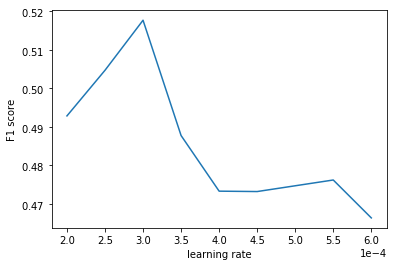
\includegraphics[scale=0.58]{agent_local_avg_f1.png}
    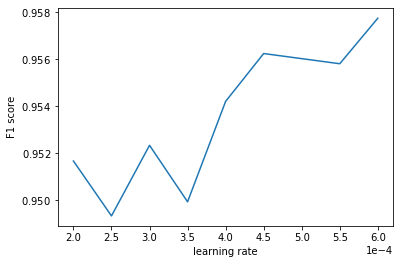
\includegraphics[scale=0.58]{clock_score_avg_f1.png}
    \caption{Probe F1 scores averages on agent localization variables (left) and score/clock variables (right) for different learning rates of the encoder on the Boxing game}
    \label{fig:agent_local_avg_f1}
\end{figure}

In Figure \ref{fig:agent_local_avg_f1}, we see that the $\alpha=0.3$ learning rate used in the article is the optimal value for the agent localization variables, but not for the score/clock variables. This suggests that an ensemble of encoders can be trained to predict a particular category of variables, and this would allow for an optimal learning rate for each category of variables instead of having a global learning rate applied on a single encoder. However, this idea implies training five encoders instead of one.\\

After this tuning process, we explored some different parameters of the encoder. Every training was realised with the same learning rate $\alpha=0.3$. \\

\begin{SCfigure}[][h]
    \centering
    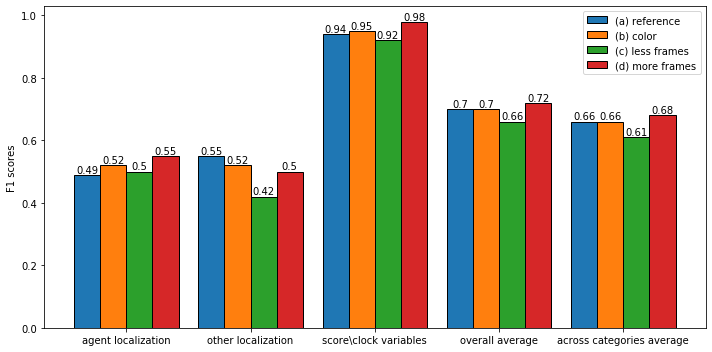
\includegraphics[scale=0.45]{multiple_params_testing.png}
    \caption{Exploration of different parameters for the encoder on the Boxing game. (a) refers to the base encoder with the default parameters (grayscaling, and trained on $100000$ frames). (b) refers to the model (a) without grayscaling. (c) and (d) refer to the model (a) but trained on respectively $50000$ and $150000$ frames. The probe F1 scores are reported for different categories.}
    \label{fig:multiple_params}
\end{SCfigure}

In Figure \ref{fig:multiple_params}, comparing (a) and (b) allows us to confirm that applying grayscaling to the frames does not impact the results. The results obtained with (a), (c) and (d) show that the default size of $100000$ for the number of frames the model is trained on was well chosen. Indeed, taking less frames leads to worse results and taking more frames leads to very similar results. This parameter is important because in addition to affecting the accuracy of the encoders, they greatly impact the training time: (d) took around $15$ hours to train as opposed to $10$ hours for (a).

\subsection{Modifying the Loss Function}
For our second ablation we modify and test the STDIM loss function by weighting the global-local and local-local objectives by a factor $p\in \left[0, 1\right]$:
\begin{equation}
\mathcal{L}=p\cdot\mathcal{L}_{GL}+(1-p)\cdot\mathcal{L}_{LL}
\end{equation}
By varying $p$, we re-weight the importance of minimizing either objective's loss, and by setting $p=0.5$ they will be weighted equally, and thus the loss is equivalent to the standard STDIM loss. This ablation is similar to an ablation by Anand et. al which contrasts the global output of the encoder at both time steps, hence creating a new global-global objective based on InfoNCE \cite{main_article}. Moreover, their codebase includes code which implements the $p=1$ case of this loss, however this ablation wasn't explicitly mentioned in their article.

\begin{figure}[H]
    \centering
    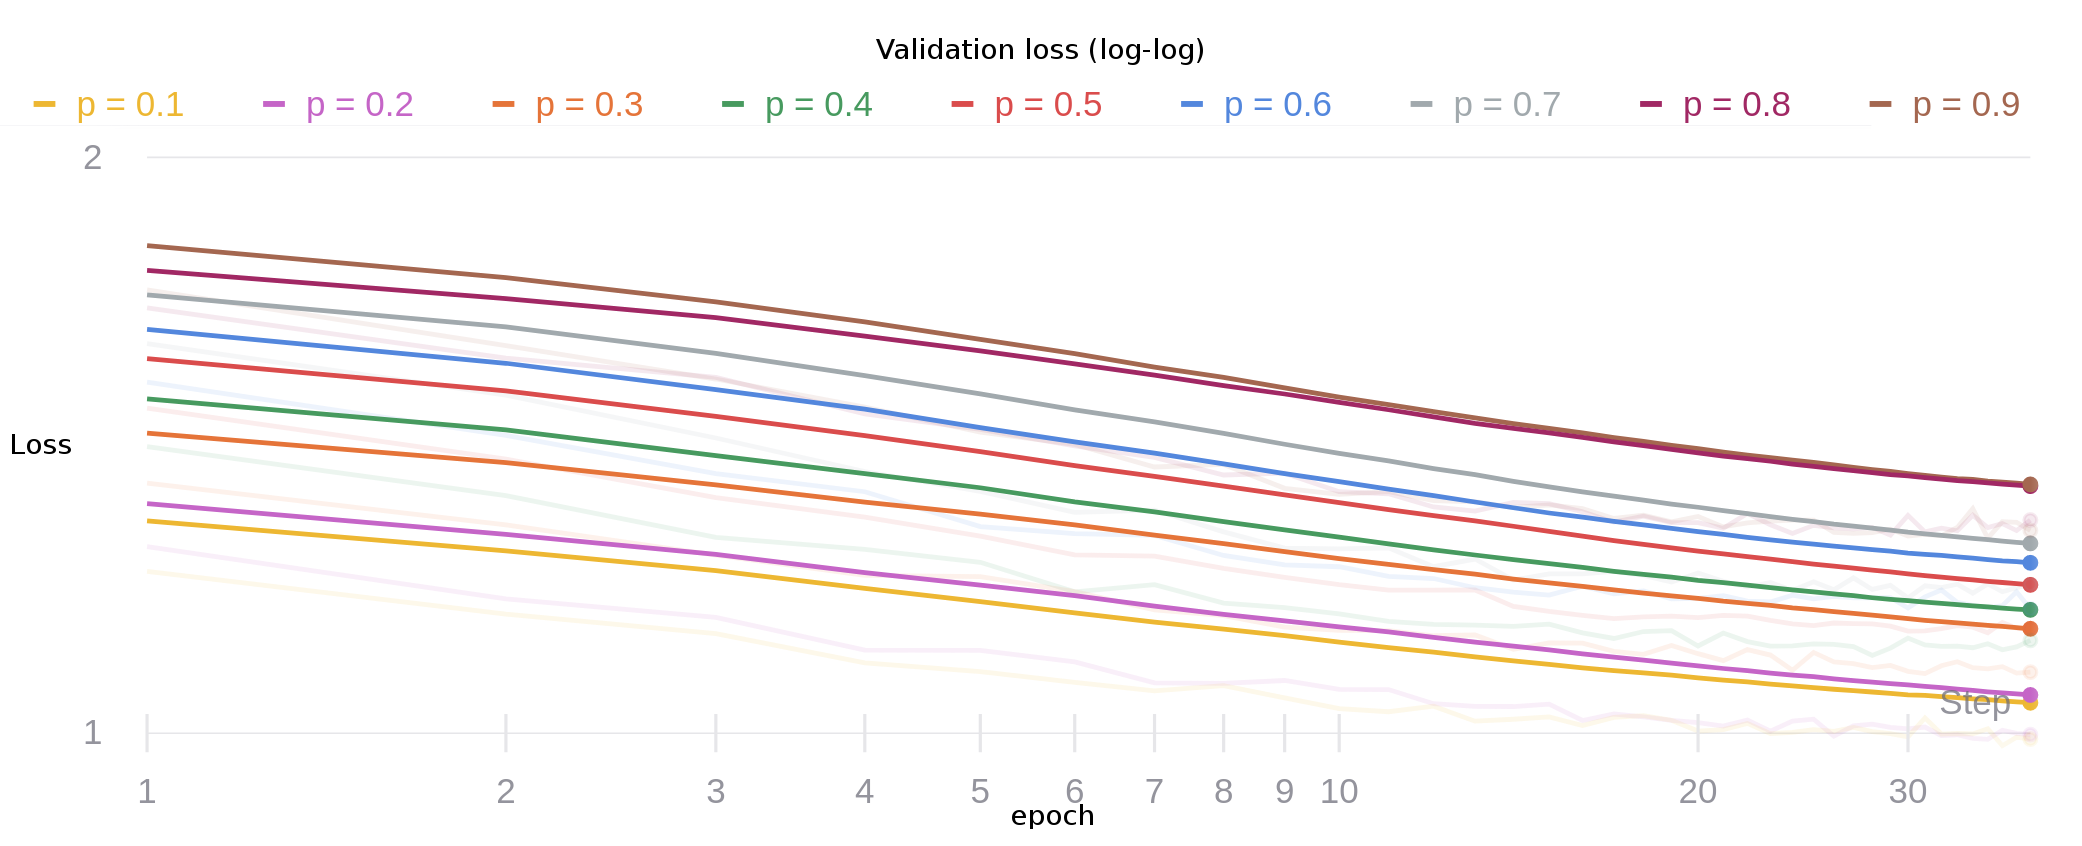
\includegraphics[scale=0.23]{ablation2-val_loss(log-log).png}
    \caption{Log-log plot of the validation loss of the trainer over time.}
    \label{fig:ablation2-loss}
\end{figure}

As our initial hypothesis would suggest, the loss seemed to have general trend of being smaller as $p$ does so as well for, as seen in Figure \ref{fig:ablation2-loss}. All $p$ value losses converge at roughly the same rate and differ by a constant as expected.

\begin{figure}[H]
    \centering
    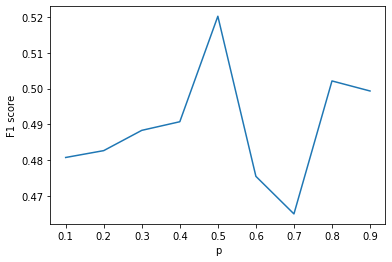
\includegraphics[scale=0.38]{ablation2-agent_avg_f1.png}
    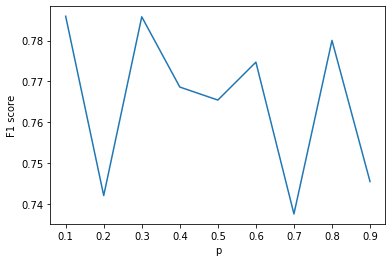
\includegraphics[scale=0.38]{ablation2-score_avg_f1.png}
    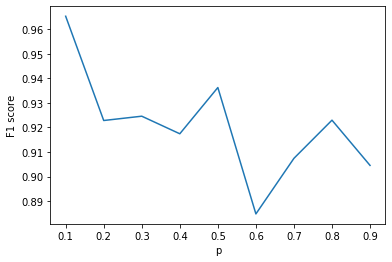
\includegraphics[scale=0.38]{ablation2-other_avg_f1.png}
    \caption{Probe F1 scores averages from Space Invaders on agent localization variables (left), score/clock variables (center) and other (right) for different values of $p$}
    \label{fig:ablation2-avg}
\end{figure}

As seen in the left of Figure \ref{fig:ablation2-avg}, a balanced loss for agent probing is by far the best, with both sides lower, $p=0.5$ stands out as the best value. For scoring and miscellaneous variables, this is not as clear. The balanced loss is generally among the top values however, extreme values are able to outperform in certain categories. In the case of score/clock variables, either extreme is capable of achieving higher scores. As for miscellaneous states, on the right of Figure \ref{fig:ablation2-avg}, this trend suggests that highly weighting the global local objective exhibits better performance in general. \\

Unfortunately, these conclusions are based only on 9 runs and a single game. To get clearer trends, this cycle should be performed multiple times on each $p$ value for more $p$ values to get an idea for the variation of p. However, we are still quite within our means to come to the conclusion that a different encoder for each category of variables would be most beneficial as each category suggests to follow different trends. \\

An avenue for future research would be to experiment with increasing the number of frames used in the score function. Doing this would require extending the definition of the InfoNCE objective to three variables.
\begin{equation}
\mathcal{I}_{NCE}=\sum_{i=1}^N\log{\frac{\exp{f(x_i,x_{i+1},x_{i+2})}}{\sum\limits_{\substack{j_1}}\sum\limits_{\substack{j_2}} \exp{f(x_i,x_{j_{1}},x_{j_{2}})}}}
\end{equation}
In STDIM, a window of three consecutive frames $(x_t, x_{t+1},x_{t+2})$ would constitute a positive sample, and  the function $f$ would take three frames. However it's unclear if this extension would yield linearly interpretable representations as effectively as the bivariate case of InfoNCE as introduced by van den Oord \cite{infoNCE}.

\subsection{Modifying the Receptive Field of the Base Encoder}
\label{section:receptive-field}

Our final ablation was to explore the effect of tuning the receptive field size of the encoders when computing the loss in equation \ref{eqn:loss-functions}. Anand et. al use a receptive field size of $1/16$ without justification in the paper \cite{main_article}. The selection of the intermediate layer which defines $\phi_{m,n}$ in the bilinear score functions for the STDIM loss is fixed such that the receptive field of that layer is $1/16^{th}$ of the original image. In our experiments we kept the layer we used fix, but we modified the strides of the base encoder from Figure \ref{fig:base-encoder-image} to achieve receptive field sizes of $1/8$ and $1/32$.

The default strides used in the network are $4, 2, 2, 1$, and thus the third convolutional layer has a receptive field size of $1/16$. For testing a receptive field size of $1/8$ we employ the strides $4, 2, 1, 2$, thus ensuring the output size is approximately the same barring padding. To accomplish $1/32$ we employ the strides $4, 4, 2, 1$, and to compensate for greatly reducing the size of the output of the final convolutional layer we change its depth from $64$ to $128$.

\begin{table}[H]
\centering
\begin{tabular}{ll}
    \begin{tabular}{c|ccc}
         \toprule Receptive field size & 1/8 & 1/16 & 1/32 \\
         \hline MontezumaRevenge & \textbf{0.83} & 0.80 & 0.73  \\
         MsPacman & 0.72 & \textbf{0.72} & 0.72 \\
         Pong & 0.81 & \textbf{0.84} & 0.68 \\
         SpaceInvaders & 0.60 & \textbf{0.61} & 0.59 \\
         Pitfall & \textbf{0.62} & 0.59 & 0.57 \\\bottomrule
    \end{tabular}
&

    \begin{tabular}{c|ccc}
        \toprule Receptive field size & 1/8 & 1/16 & 1/32 \\
        \hline Agent Localization & 0.55 & \textbf{0.57} & 0.43 \\
        Other Localization & \textbf{0.81} & 0.80 & 0.76 \\
        Score/Clock/Lives/Display & 0.93 & \textbf{0.94} & 0.91 \\
        Small object Localization & 0.53 & \textbf{0.54} & 0.53 \\
        Miscellaneous & \textbf{0.68} & 0.65 & 0.60 \\\bottomrule
    \end{tabular}
\end{tabular}
\caption{Probe F1 scores averaged across all categories for the various receptive field sizes (left) and averaged over all games by receptive field size (right). The bold numbers represent the best result.}
\label{tab:receptive-field-results}
\end{table}

Table \ref{tab:receptive-field-results} summarizes the results of this ablation. Training an encoder for $1/8$ receptive field takes approximately 4 times as long due to there being twice as many spatial locations to compute the loss for in each dimension. Therefore due to compute time constraints we evaluated on a subset of 5 games which contain a significant diversity in variable types. These results validate that $1/16$ was a good choice of receptive field by the authors, however $1/8$ seems to perform better for variables in the \textbf{Other Localization} and \textbf{Miscellaneous} categories. The results match closely for both $1/8$ and $1/16$ receptive field sizes, and thus both seem to be viable options for training encoders. As expected, $1/ 32$ performs poorly as the mutual information estimate is based off large patches of the original image, and thus the encoder focuses on only a few locations in the image. \\

An interesting direction for future work would be to experiment with adding multiple STDIM objectives based on various layers of the encoder, such that the loss hinges on multiple receptive field sizes.

\begin{equation}
\mathcal{L}=\sum_{\ell}\mathcal{L}^{(\ell)}_{GL}+\mathcal{L}^{(\ell)}_{LL}=\sum_{\ell}\sum_{m=1}^M\sum_{n=1}^N-\left(\log{\frac{\exp{g^{(\ell)}_{m,n}(x_t,x_{t+1})}}{\sum\limits_{\substack{x_t^\star}} \exp{g^{(\ell)}_{m,n}(x_t,x_t^\star)}}}+\log{\frac{\exp{f^{(\ell)}_{m,n}(x_t,x_{t+1})}}{\sum\limits_{\substack{x_t^\star}} \exp{f^{(\ell)}_{m,n}(x_t,x_t^\star)}}}\right)
\label{eqn:loss-functions-over-layers}
\end{equation}

where each score function $g^{\ell}_{m,n}$ and $f^{\ell}_{m,n}$ are defined using bi-linear functions as in equation \ref{eqn:bilinear} but $\phi_{m,n}$ is based on layer $\ell$ of the encoder. This would force the encoder to jointly maximize the mutual information of its representation at each of these receptive field sizes.

\section{Discussion and Conclusion}
Thanks to the efforts of the authors in making their code accessible and interpretable, the results obtained in their article were easily reproducible. We must point out the fact that noteworthy computational power is necessary for reproducing results and to investigate further. It took $17$ days of total compute time to obtain all the results in this report with our limited computational power.\\

We noticed that the authors made choices about the architecture of the encoder, namely the receptive field size and the equal weighting of the GL and LL objectives, without explaining some of the theoretical motivations behind them. For instance, the $1/16$ receptive field decision took up $1$ sentence in the paper, and we believe that decision merits more exploration. To best complement their work, we focused our ablations on ideas that we felt were under explored. Our results showed that the author's decisions with regards to those ablations were experimentally sound. However, bearing in mind that most of the final results stated throughout this study come from the evaluation of a single encoder, these don't fully prove the strength of the aforementioned decisions. For instance, it is much more likely to see a meaningful trend in the performance of the encoders as a function of $p$ if we train multiple times over all $22$ games and average the performances. \\

For future work, the first thing to do would be to repeat our experiments using a larger sample size in order to reduce variance. Also training an ensemble of different encoders for each category of variables, selecting ablations discussed in Section 5 with respect to the best choice for each category. We would also explore the various modifications to the loss as described in Sections 5.2 and 5.3.

\section{Acknowledgements}
We would like to thank Ankesh Anand who gave us some hints and paths to explore at the beginning of our project, and was generally supportive by answering all of our questions throughout the process. We also thank our girlfriends who gave us all of their free Google Cloud Platform credits.

\bibliographystyle{plain}
\bibliography{bibliography}
\end{document}
